\documentclass[11pt]{article}
\usepackage[english]{babel}
\usepackage[latin1]{inputenc}
\usepackage{amsmath,amssymb,amsfonts,latexsym,graphicx,color}
\textwidth16cm \textheight22cm \voffset-0.8cm \hoffset-2cm
\DeclareMathOperator{\sgn}{sgn}
\DeclareMathOperator{\Tr}{Tr}
\DeclareMathOperator{\Rea}{Re}
\DeclareMathOperator{\Ima}{Im}
\def\bbm[#1]{\mbox{\boldmath $#1$}}
\newcommand{\ket}[1]{\displaystyle{|#1\rangle}}
\newcommand{\bra}[1]{\displaystyle{\langle #1|}}
\newcommand{\TE}{\text{TE}}
\newcommand{\TM}{\text{TM}}

\begin{document}

\section{Convective cooling}

\subsection{Geometrical definitions and injected power}

Suppose we have a chip made of $N_\mathrm{cores}$ cores. Each of these has thickness $\delta$ along the $z$ axis and a total area $A_\mathrm{core}$. Part of this area $A_\mathrm{FU}$ is a region (a functional unit) where a potentially higher power density is injected and might thus experience a hotspot generation.

The power injected into the area $A_\mathrm{core}$ ($A_\mathrm{FU}$) is defined as $P_\mathrm{core}$ ($P_\mathrm{FU}$). This implies that the total power injected in the entire system reads $P_\mathrm{inj} =  P_\mathrm{core} + P_\mathrm{FU}$.

\subsection{Convective cooling power}

We assume that one or several fans are operating to cool the chip. These fans are blowing air inside the system at a given fan speed $v_\mathrm{air}$. We assume that the function relating this speed to the power needed to operate the fans is known and defined as $P_\mathrm{fan}(v_\mathrm{air})$. As a matter of fact, our calculations are based on the knowledge of this power--speed curve for three different models of fan, operating in three different regions of air speeds. The data extracted from the data sheets are shown in Fig.~\ref{Fan_power}(a), along with the associated linear fitting curves. We will assume in the following that for a given air speed, the best fan is chosen, so that the cumulative power--speed curve is the one shown in Fig.~\ref{Fan_power}(b).

\begin{figure}[h!]
	\centering
	\includegraphics[width=0.45\textwidth]{Fan_power_1}
	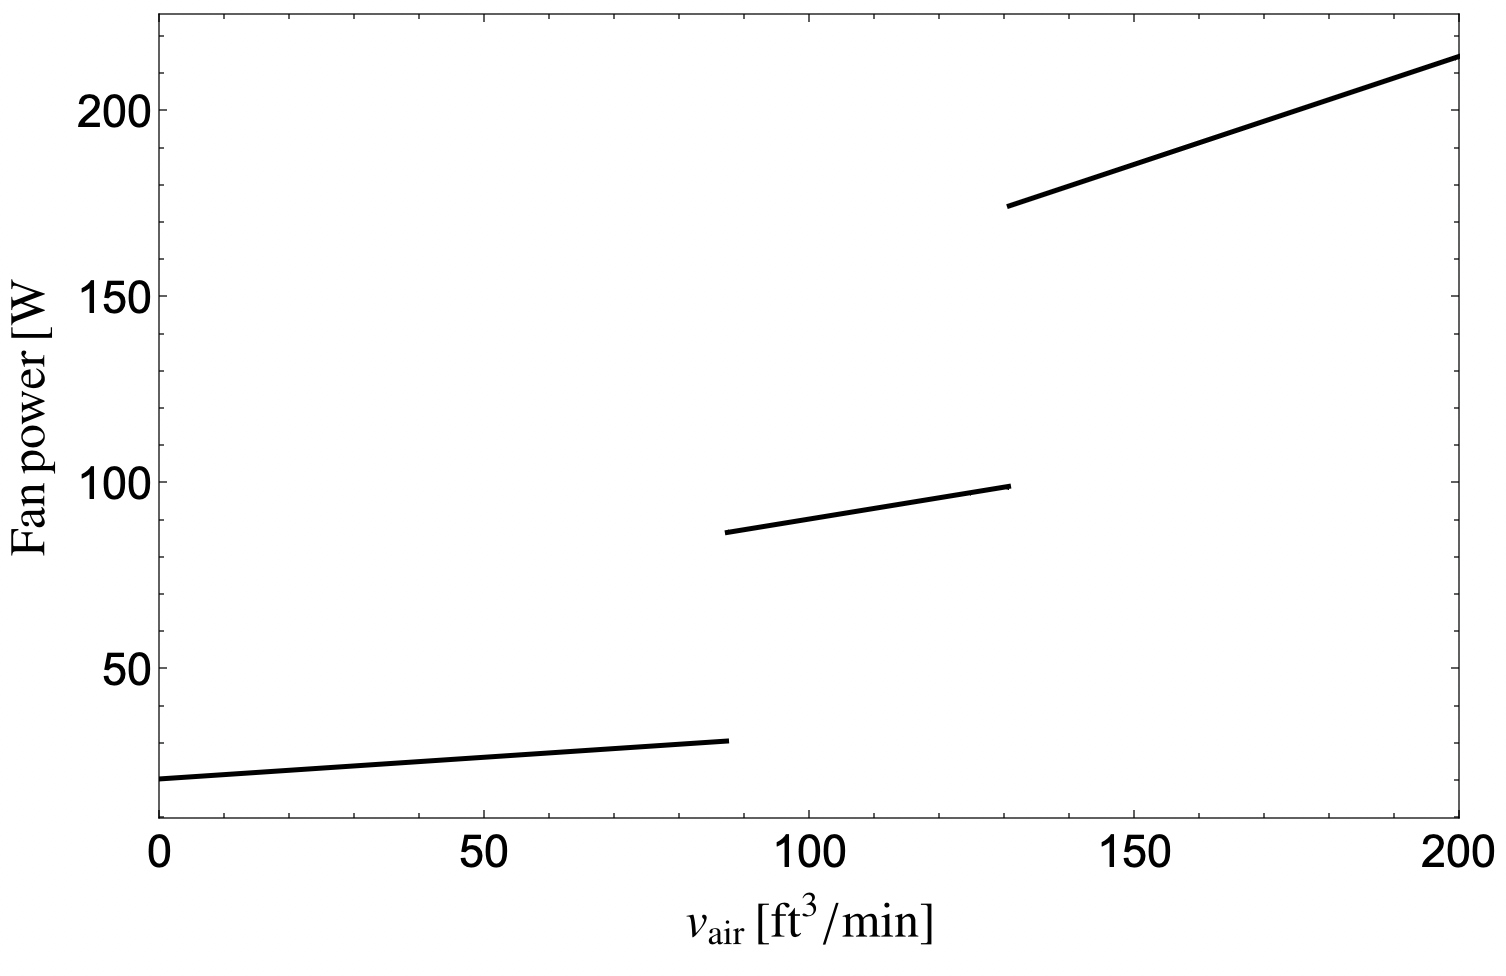
\includegraphics[width=0.45\textwidth]{Fan_power_2}
	\caption{(a) Data extracted from the data sheets of three different fans along with the associated linear fit. (b) Cumulative power--speed curve assuming that the best fan is chosen for each value of the air speed.} \label{Fan_power}
\end{figure} 

\subsection{Laser cooling power}

We assume that a localized heat-sink region is placed in proximity to each functional unit. A total power $P_\mathrm{extr}$ is extracted at these heat-sink regions. This results in delivering an external laser power $P_\mathrm{laser}=\eta_\mathrm{laser} P_\mathrm{extr}$

\subsection{Coefficient of performance}

For our system we define a coefficient of performance (COP) as
\begin{equation}
	\mathrm{COP} = \frac{P_\mathrm{inj} + P_\mathrm{cooling}}{P_\mathrm{cooling}} =  \frac{P_\mathrm{inj} + P_\mathrm{fan}(v_\mathrm{air}) + \eta_\mathrm{laser} P_\mathrm{extr}}{P_\mathrm{fan}(v_\mathrm{air}) + \eta_\mathrm{laser} P_\mathrm{extr}}.
\end{equation}

\subsection{Maximum chip temperature vs injected power}

Within SimScale we have simulated the maximum temperature within the entire chip as a function of the injected power. This has been done for several values of the convective air speed, ranging from 10 to 200 ft$^3$/m, and by varying independently the powers $P_\mathrm{core}$ and $P_\mathrm{FU}$ injected in the core and functional-unit regions, respectively. For each given fan speed two different procedures are followed. The former consists in varying both $P_\mathrm{core}$ and $P_\mathrm{FU}$. In this scenario the results obtained for the maximum chip temperature are fitted bi-linearly as a function of $P_\mathrm{core}$ and $P_\mathrm{FU}$ according to the expression
\begin{equation}
	T_\mathrm{max}(v_\mathrm{air},P_\mathrm{core},P_\mathrm{FU}) = T_0 + \alpha_\mathrm{on}(v_\mathrm{air})P_\mathrm{core} + \beta_\mathrm{on}(v_\mathrm{air})P_\mathrm{FU},
\label{Fit_on}\end{equation}
where $T_0=19.85^\circ$C is the reference temperature used for air in our simulation. Our second scenario consists in varying only $P_\mathrm{core}$ and keeping $P_\mathrm{FU}=0$. The corresponding results are fitted linearly according to
\begin{equation}
	T_\mathrm{max}(v_\mathrm{air},P_\mathrm{core},P_\mathrm{FU}) = T_0 + \alpha_\mathrm{off}(v_\mathrm{air})P_\mathrm{core}.
\label{Fit_off}\end{equation}
The subscript ``off" refers here to switching off the potential hotspot appearing at the locations of the functional units. These results are assumed to correspond to the scenario in which a heat sink is balancing exactly the power $P_\mathrm{FU}$ injected at the functional units. This has also been verified independently through simulations with $P_\mathrm{core}$ and $P_\mathrm{FU}$ both present and an extracted power $P_\mathrm{extr}=P_\mathrm{FU}$.

\begin{figure}[h!]
	\centering
	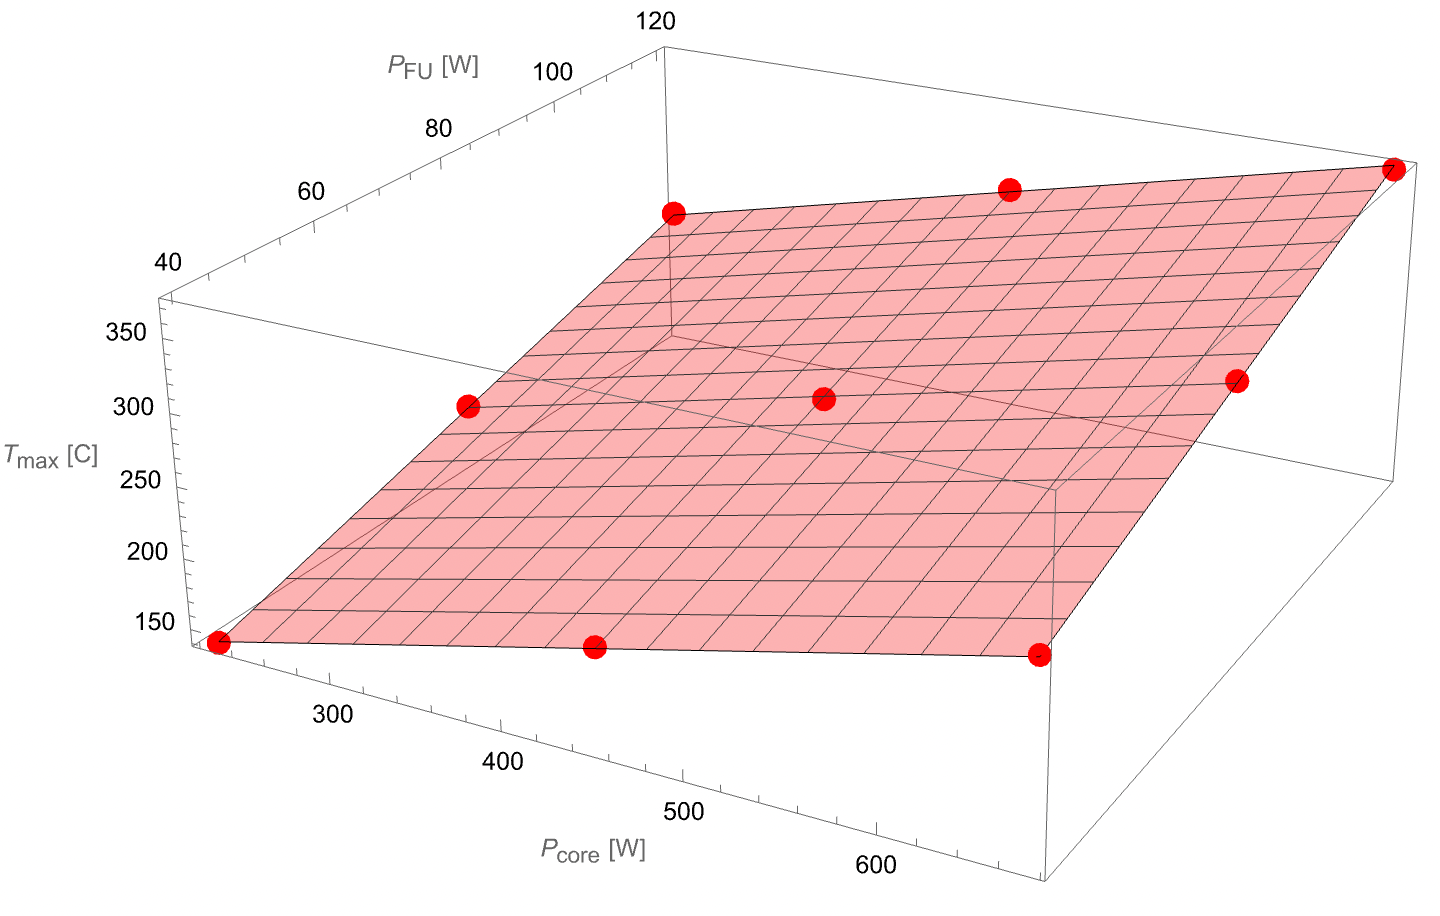
\includegraphics[width=0.75\textwidth]{Tmax_fit}
	\caption{Simulated maximum chip temperature as a function of the injected core and functional-unit powers, along with the bi-linear and linear fits. The red data correspond to the ``on" scenario ($P_\mathrm{core}$ and $P_\mathrm{FU}$ both different from zero), whereas the black data correspond to the ``off" scenario ($P_\mathrm{FU}$=0). The data shown here correspond to $v_\mathrm{air}=70\,\mathrm{ft}^3/\mathrm{min}$} \label{Tmax_fit}
\end{figure}

The coefficients $\alpha_\mathrm{on}(v_\mathrm{air})$ , $\beta_\mathrm{on}(v_\mathrm{air})$  and $\alpha_\mathrm{off}(v_\mathrm{air})$ are shown in Fig.~\ref{Coefficients}. While these coefficients decrease as expected when increasing air speed, mitigating the impact of increased injected power on the maximum chip temperature, it is important to highlight a clear saturation effect when going toward the highest values of the air speed, proving the limitations of air cooling.

\begin{figure}[h!]
	\centering
	\includegraphics[width=0.75\textwidth]{Coefficients}
	\caption{Fitting coefficients defined in Eqs.~\eqref{Fit_on} and \eqref{Fit_off} as a function of the air speed. The $\alpha$ coefficients for the ``on" and ``off" scenarios are almost superposed.} \label{Coefficients}
\end{figure}

\subsection{Combined effect of air and laser cooling}

We now exploit the knowledge of these coefficients to analyze the combined impact of air and laser cooling. As stated above, we assume that the ``off" scenario corresponds to the results we would get by extracting an amount of energy $P_\mathrm{extr}=P_\mathrm{FU}$ equal to the one injected at the functional units. Moreover, we assume that for extracted powers $0<P_\mathrm{extr}<P_\mathrm{FU}$ between the two extreme values, a linear behavior of the maximum chip temperatures can be assumed. This has also been verified numerically within SimScale with simulations involving a varying extracted power. We finally recall that extracting a given power $P_\mathrm{extr}$ amounts to spend a laser power $P_\mathrm{laser}=\eta_\mathrm{laser}P_\mathrm{extr}$.

We are now ready to express the maximum chip temperature as a function of the air speed $v_\mathrm{air}$, the laser power $P_\mathrm{laser}$ and the injected powers $P_\mathrm{core}$ and $P_\mathrm{FU}$. The final expression reads
\begin{equation}\begin{split}
	T_\mathrm{max}(v_\mathrm{air},P_\mathrm{laser},P_\mathrm{core},P_\mathrm{FU}) &= T_0 + \Bigl[\alpha_\mathrm{on}(v_\mathrm{air})+\frac{P_\mathrm{laser}}{\eta_\mathrm{laser}P_\mathrm{FU}}(\alpha_\mathrm{off}(v_\mathrm{air})-\alpha_\mathrm{on}(v_\mathrm{air}))\Bigr]P_\mathrm{core}\\
	&\,+\beta_\mathrm{on}(v_\mathrm{air})\Bigl(1-\frac{P_\mathrm{laser}}{\eta_\mathrm{laser}P_\mathrm{FU}}\Bigr)P_\mathrm{FU}.
\end{split}\label{Tmax_full}\end{equation}

This expression is used to plot in Fig.~\ref{ContourPlot} the maximum chip temperature $T_\mathrm{max}$ as a function of the laser input power $P_\mathrm{laser}$ and air speed $v_\mathrm{air}$ for $P_\mathrm{core}=290\,$W and $P_\mathrm{FU}=70\,$W. If we focus for example on a given contour line, say the one at $T_\mathrm{max}=150^\circ$C, we remark that by increasing the laser power a lower air speed is needed to keep the chip at a given temperature. Moreover, we remark that for some temperatures (e.g. $T_\mathrm{max}=150^\circ$C) air cooling is simply unable to keep the chip at a given temperature in the absence of laser cooling.

\begin{figure}[h!]
	\centering
	\includegraphics[width=0.5\textwidth]{Contour_plot}
	\caption{Maximum chip temperature $T_\mathrm{max}$ as a function of laser power $P_\mathrm{laser}$ and air speed $v_\mathrm{air}$ for $P_\mathrm{core}=290\,$W and $P_\mathrm{FU}=70\,$W.} \label{ContourPlot}
\end{figure}

\subsection{Impat of laser cooling on COP}

The knowledge of the full dependence given in Eq.~\eqref{Tmax_full} of $T_\mathrm{max}$ on all parameters allows us to raise the two following questions. If the injected powers $P_\mathrm{core}$ and $P_\mathrm{FU}$ are known and we want to operate at a given chip temperature, is it possible to do that without laser cooling? In the presence of laser cooling, what is its value producing the highest possible COP? The answer can be obtained by following the contour line corresponding to the desired temperature in Fig.~\ref{ContourPlot} and following the corresponding COP, thanks to the knowledge of the fan power as a function of air speed given by Fig.~\ref{Fan_power}(b). Figure \ref{Fig_COP}(a) shows the total cooling power needed to operate at either 150$^\circ$C or 180$^\circ$C as a function of the laser power, while Fig.~\ref{Fig_COP}(b) shows the associated COP. We see that operating at 150$^\circ$C without laser cooling is simply impossible (the blue curve starts at $P_\mathrm{laser}\simeq50\,$W) and that the best COP is realized at a value of the laser power higher than the minimum. This corresponds to a value for which a transition toward the most efficient fan is realized. On the contrary, it is indeed possible to operate at 180$^\circ$C without laser cooling and moreover the best COP is realized in this scenario when the laser is switched off. The reason is that at such temperature, even without laser cooling, air cooling is operating with its most efficient fan.

\begin{figure}[h!]
	\centering
	\includegraphics[width=0.45\textwidth]{COP_1}
	\includegraphics[width=0.45\textwidth]{COP_2}
	\caption{(a) Total cooling power and (b) COP as a function of the laser power for $P_\mathrm{core}=290\,$W and $P_\mathrm{FU}=70\,$W, at two operating temperatures (see legend).} \label{Fig_COP}
\end{figure}

We conclude with a different set of questions: suppose we want our chip to operate at a given temperature, say 100$^\circ$C. Both in the absence and in the presence of laser cooling, what is the range of injected powers $P_\mathrm{core}$ and $P_\mathrm{FU}$ allowing this and at which COP? The answer is given in Fig.~\ref{Fig_2D}.

The left panel shows the scenario without laser cooling. It can be clearly seen that air cooling cannot make the chip operate at 100$^\circ$C outside a limited region of $P_\mathrm{core}$ and $P_\mathrm{FU}$. Moreover, the COP rapidly decreases to values around 1 when approaching this boundary. On the contrary, the right panel shows the scenario with laser cooling. Each point corresponds to the best possible COP as a function of the applied laser power. While the region close to low values of $P_\mathrm{core}$ and $P_\mathrm{FU}$ resembles the one in the absence of laser cooling (in that range there is no benefit of adding laser cooling), it is clear that laser cooling allows to keep the temperature controlled at 100$^\circ$C and increase significantly both injected powers.

\begin{figure}[h!]
	\centering
	\includegraphics[width=0.45\textwidth]{Fig_2D_1}
	\includegraphics[width=0.45\textwidth]{Fig_2D_2}
	\caption{Cooling COP to make the chip operate at 100$^\circ$C in the absence (left) and presence (right) of laser cooling.} \label{Fig_2D}
\end{figure}

\end{document}

